\chapter{各尺度上的生物多样性}\label{ch:g10:biodiversity-scales}

在草坪上围出一个一米见方的绳框，数一数框内长着什么：
草当然有，还有三叶草、雏菊、一株蒲公英、车前草、苔藓；
若用放大镜细看，还能找到十几只昆虫和一只蜗牛。
把方框移到停车场的柏油路面上：什么也没有，或者只有裂缝里的一株杂草。
把它移到一片从未被耕作过的老草甸：四十种植物，
还有数不清的昆虫。这个方框所测量的，就是\emph{\omterm{def:g10:biodiversity-scales:biodiversity}{生物多样性}}。
本章要讨论的是如何测量它、
它存在于哪些尺度上，
以及它为何既不固定，也无法保证。

\section{多样性的三个尺度}

\begin{definition}[生物多样性]\label{def:g10:biodiversity-scales:biodiversity}
\emph{生物多样性}\index{生物多样性}是指生物界的多样性，
从以下三个尺度来考察：
\begin{itemize}
  \item \emph{生态系统}\index{生态系统}的多样性——
        生物群落及其所处环境的多样性（如池塘、山毛榉林、珊瑚礁、草地），
        每个生态系统各有其特定的
        \omterm{def:g10:biodiversity-scales:species}{物种}组成；
  \item 生态系统内或地球上\omterm{def:g10:biodiversity-scales:species}{物种}的多样性——
        \omterm{def:g10:biodiversity-scales:species}{物种}的数目及其
        相对丰度；
  \item \omterm{def:g10:biodiversity-scales:species}{物种}内部的\emph{遗传多样性}\index{遗传多样性}——
        即其\omterm{def:g10:universal-dna:gene}{基因}的\omterm{def:g10:universal-dna:gene}{等位基因}数目，
        以及这些\omterm{def:g10:universal-dna:gene}{等位基因}在个体与种群之间的分配方式。
\end{itemize}
\end{definition}

\begin{omfigure}
\begin{tikzpicture}[font=\small, >=Stealth]
  \node[draw, rounded corners, thick, fill=omMeth!8, minimum width=11.4cm, minimum height=4.9cm] (eco) at (0,0) {};
  \node[anchor=north west, font=\small\bfseries] at (eco.north west) {\ 生态系统：池塘、林地、珊瑚礁、草地\dots};
  \node[draw, rounded corners, thick, fill=omDef!10, minimum width=8.2cm, minimum height=3.2cm] (sp) at (0.6,-0.45) {};
  \node[anchor=north west, font=\small\bfseries] at (sp.north west) {\ 某一生态系统中的物种};
  \foreach \x/\t in {-2.6/蛙, -1.1/蝾螈, 0.4/蜻蜓, 1.9/芦苇, 3.4/睡莲}
    \node[draw, fill=white, rounded corners=2pt, font=\scriptsize] at (\x,-0.3) {\t};
  \node[draw, rounded corners, thick, fill=omProp!12, minimum width=6.4cm, minimum height=1.2cm] (al) at (1.0,-1.35) {};
  \node[anchor=west, font=\scriptsize\bfseries] at (al.west) {\ 某一物种的等位基因：};
  \foreach \x/\t in {1.6/a, 2.2/b, 2.8/c, 3.4/d, 4.0/e}
    \node[draw, circle, fill=white, inner sep=1.5pt, font=\scriptsize] at (\x,-1.35) {\t};
\end{tikzpicture}

{\small \omterm{def:g10:biodiversity-scales:biodiversity}{生物多样性}的三个嵌套尺度。失去一个池塘，就失去一个群落；
失去一个\omterm{def:g10:biodiversity-scales:species}{物种}，就失去它的全部\omterm{def:g10:universal-dna:gene}{等位基因}；失去\omterm{def:g10:universal-dna:gene}{等位基因}，
则使仍然存在的\omterm{def:g10:biodiversity-scales:species}{物种}变得贫乏。}
\end{omfigure}

\begin{definition}[物种]\label{def:g10:biodiversity-scales:species}
\emph{物种}\index{物种}是指外形相似、
能够相互交配并产生可育后代的一类生物；两个
不能杂交、或杂交后代不育的种群，
则属于不同的物种。实际上——对于化石、细菌，
或从未观察到交配的生物而言——物种是依据其共有特征来识别的，
而\cref{ch:g12:selection-drift-speciation}
将说明，物种之间的界限并不总是清晰的。
\end{definition}

\begin{example}[马、驴与骡]\label{ex:g10:biodiversity-scales:mule}
马与驴外形相似，能够相互交配，
其后代为骡。但骡不育，因此马和驴是两个\omterm{def:g10:biodiversity-scales:species}{物种}。
贵妇犬与猎狼犬外形毫不相像，却能相互交配，
并产下可育的幼犬：二者同属一个\omterm{def:g10:biodiversity-scales:species}{物种}，即犬——
它也能与其祖先狼交配。
\end{example}

\section{物种的多样性}

\begin{proposition}[物种计数]\label{prop:g10:biodiversity-scales:count}
目前已描述并命名的\omterm{def:g10:biodiversity-scales:species}{物种}约有两百万种。其中大多数是昆虫
（超过一百万种），其次是植物（约 300\,000 种）、真菌、
蛛形纲动物和软体动物；脊椎动物是我们了解最多的一类，
约有 70\,000 种，其中哺乳动物有 6\,400 种。尚未被描述的\omterm{def:g10:biodiversity-scales:species}{物种}数目，
依据新\omterm{def:g10:biodiversity-scales:species}{物种}的发现速率估计，还要再多出数百万种——
全部真核生物\omterm{def:g10:biodiversity-scales:species}{物种}或许有八百万至一千万种，
此外还有数量庞大、大多未被统计的
细菌多样性。
\end{proposition}
\admitted

\begin{omfigure}
\begin{tikzpicture}
\begin{axis}[
  xbar, bar width=7pt,
  width=0.8\linewidth, height=6.4cm,
  axis x line=bottom, axis y line=left,
  xmin=0, xmax=1200,
  xlabel={已描述物种数（千）},
  xlabel style={font=\small, at={(axis description cs:0.5,-0.1)}, anchor=north},
  symbolic y coords={mammals, birds, fish, molluscs, arachnids, fungi, plants, insects},
  ytick=data, yticklabels={哺乳动物, 鸟类, 鱼类, 软体动物, 蛛形动物, 真菌, 植物, 昆虫}, tick label style={font=\small},
  enlarge y limits=0.1,
  nodes near coords, nodes near coords style={font=\scriptsize, anchor=west},
  xtick={0,200,400,600,800,1000,1200},
] 
\addplot[fill=omDef!55, draw=omDef] coordinates
  {(6.4,mammals) (11,birds) (34,fish) (85,molluscs) (100,arachnids)
   (150,fungi) (300,plants) (1000,insects)};
\end{axis}
\end{tikzpicture}

{\small 若干大类中已描述的\omterm{def:g10:biodiversity-scales:species}{物种}数，单位为千。我们了解最多的
类群恰恰是数目最少的；仅昆虫的数目就以十五比一的比例
超过全部脊椎动物。}
\end{omfigure}

\begin{method}[测量一个地点的多样性]\label{met:g10:biodiversity-scales:sampling}
对一个地点从来不是整体计数，而是要\emph{取样}。
\begin{enumerate}
  \item 选取适合该生物的取样单位：测量草地植物用
        \qty{1}{m^2} 的样方，采集昆虫用网扫，
        采集蚯蚓用一筛土壤，观察鸟类用一段样线。
  \item 随机或按固定间距设置取样单位，
        并使取样数目足够多，以至于再增加一个单位对总数的影响很小。
  \item 在每个取样单位中识别并计数。样本可用两个数值来描述：
        \emph{\omterm{def:g10:biodiversity-scales:species}{物种}丰富度}，即所发现的\omterm{def:g10:biodiversity-scales:species}{物种}数目；以及
        每个\omterm{def:g10:biodiversity-scales:species}{物种}的\emph{相对丰度}——若某地点中一个\omterm{def:g10:biodiversity-scales:species}{物种}占全部个体的 95\%，
        则该地点的多样性低于十个\omterm{def:g10:biodiversity-scales:species}{物种}均匀分享个体的地点，
        即便两者的丰富度相同。
  \item 比较不同地点时，只能采用相同的方法、投入相同的努力，
        并在同一季节进行。
\end{enumerate}
\end{method}

\begin{example}[两块草坪]\label{ex:g10:biodiversity-scales:lawns}
在一块修剪过的学校草坪上设置 10 个样方：共 6 种植物，其中草类
覆盖 90\%。在与之相邻的未修剪路边草带上设置 10 个样方：共 23 个\omterm{def:g10:biodiversity-scales:species}{物种}，
单个\omterm{def:g10:biodiversity-scales:species}{物种}的占比均不超过 30\%。草带的\omterm{def:g10:biodiversity-scales:species}{物种}更丰富、分布更均匀；这一差异
并非源于土壤或气候（二者相同），而是源于修剪，
修剪清除了所有无法在贴近地面处开花的植物。
\end{example}

\begin{omfigure}
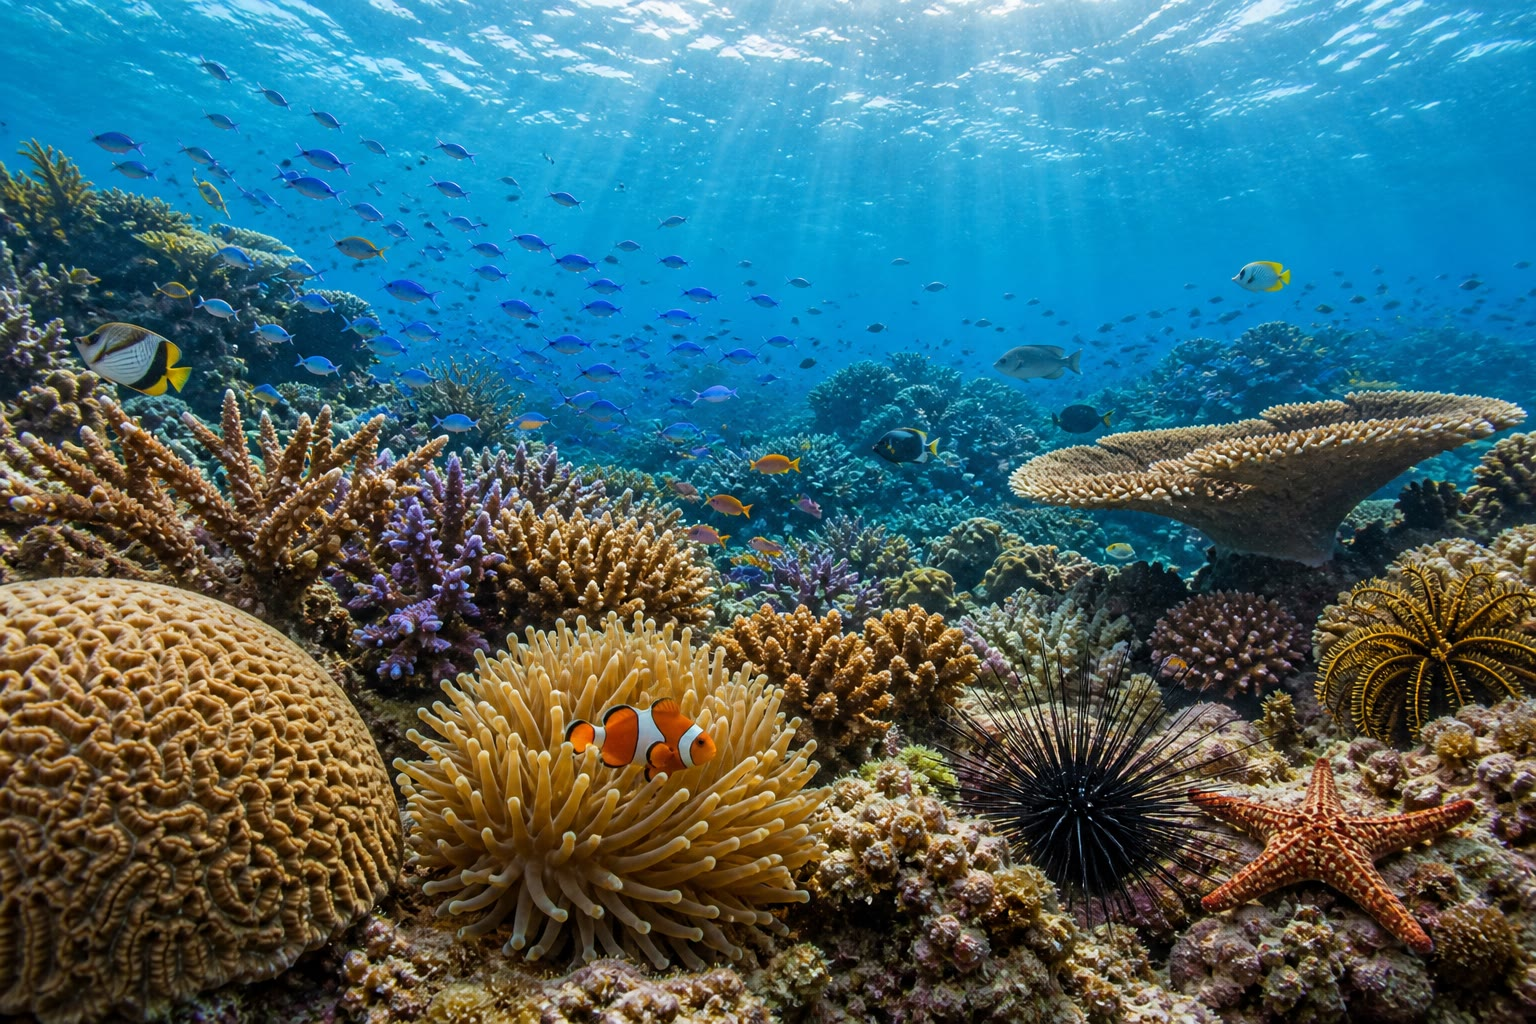
\includegraphics[width=0.66\linewidth]{images/book2/ai/g10-biodiv-coral-reef.jpg}

{\small 珊瑚礁：在几平方米内，珊瑚、鱼类、软体动物、
棘皮动物和海葵，共数十个\omterm{def:g10:biodiversity-scales:species}{物种}。珊瑚礁拥有
全部海洋\omterm{def:g10:biodiversity-scales:species}{物种}的四分之一，却只占海底面积的千分之一。}
\end{omfigure}

\section{物种内的遗传多样性}

\begin{proposition}[同一物种的个体并不相同]\label{prop:g10:biodiversity-scales:genetic}
在同一\omterm{def:g10:biodiversity-scales:species}{物种}内，大多数\omterm{def:g10:universal-dna:gene}{基因}存在多种\omterm{def:g10:universal-dna:gene}{等位基因}，而
个体所携带的\omterm{def:g10:universal-dna:gene}{等位基因}组合各不相同。
种群中某一\omterm{def:g10:universal-dna:gene}{等位基因}的\emph{频率}——即该\omterm{def:g10:universal-dna:gene}{基因}全部拷贝中
属于该\omterm{def:g10:universal-dna:gene}{等位基因}的比例——在不同种群之间
存在差异。\omterm{def:g10:biodiversity-scales:biodiversity}{遗传多样性}使\omterm{def:g10:biodiversity-scales:species}{物种}能够应对
不断变化的环境：若某种群中个体全部相同，
则自然选择便无从选择。
\end{proposition}
\admitted

\begin{example}[全球各地的血型等位基因]\label{ex:g10:biodiversity-scales:abo}
ABO 血型\omterm{def:g10:universal-dna:gene}{基因}有三种常见\omterm{def:g10:universal-dna:gene}{等位基因}：A、B 和 O。
在西欧，三者的频率约为 0.27、0.07 和 0.66；在
东亚约为 0.20、0.20 和 0.60；在南美洲部分原住民种群中，
仅 O \omterm{def:g10:universal-dna:gene}{等位基因}的频率就高达 0.98。同一\omterm{def:g10:biodiversity-scales:species}{物种}、同一
\omterm{def:g10:universal-dna:gene}{基因}，\omterm{def:g10:universal-dna:gene}{等位基因}的分布却各不相同：人类的\omterm{def:g10:biodiversity-scales:biodiversity}{遗传多样性}
是真实存在的，并且分散于各个种群之间，而非
将种群割裂开来——该\omterm{def:g10:biodiversity-scales:species}{物种}的大部分多样性
存在于任一种群之内。
\end{example}

\begin{omfigure}
\begin{tikzpicture}
\begin{axis}[
  ybar, bar width=9pt,
  width=0.8\linewidth, height=5.2cm,
  axis x line=bottom, axis y line=left,
  ymin=0, ymax=1.1, ylabel={等位基因频率}, ylabel style={font=\small},
  symbolic x coords={western Europe, eastern Asia, Andes},
  xtick=data, xticklabels={西欧, 东亚, 安第斯地区}, tick label style={font=\small},
  enlarge x limits=0.25,
  legend style={at={(0.5,-0.2)}, anchor=north, legend columns=3,
                font=\small, draw=none},
  ytick={0,0.2,0.4,0.6,0.8,1.0},
]
\addplot[fill=omThm!50, draw=omThm] coordinates {(western Europe,0.27) (eastern Asia,0.20) (Andes,0.01)};
\addplot[fill=omProp!50, draw=omProp] coordinates {(western Europe,0.07) (eastern Asia,0.20) (Andes,0.01)};
\addplot[fill=omDef!50, draw=omDef] coordinates {(western Europe,0.66) (eastern Asia,0.60) (Andes,0.98)};
\legend{等位基因 A, 等位基因 B, 等位基因 O}
\end{axis}
\end{tikzpicture}

{\small 三个人类种群中三种 ABO \omterm{def:g10:universal-dna:gene}{等位基因}的近似频率。
同一种群中三个频率之和为 1。}
\end{omfigure}

\begin{example}[几乎没有遗传多样性的物种]\label{ex:g10:biodiversity-scales:cheetah}
猎豹在遗传上高度相似，以至于无亲缘关系的个体之间
的皮肤移植，竟如同双胞胎之间一样被接受：该\omterm{def:g10:biodiversity-scales:species}{物种}
约一万年前经历过个体数极少的瓶颈，此后
便再未恢复其\omterm{def:g10:universal-dna:gene}{等位基因}。无论出现何种新疾病或新气候，
每只猎豹都以相同的“装备”去应对；该\omterm{def:g10:biodiversity-scales:species}{物种}得以存续，
但毫无储备。
\end{example}

\section{生物多样性的变化：过去与现在}

\begin{proposition}[生物多样性是一种状态，而非恒定不变]\label{prop:g10:biodiversity-scales:changes}
某一时刻存活的\omterm{def:g10:biodiversity-scales:species}{物种}集合，只是历史进程中的一个阶段。
化石记录显示，\omterm{def:g10:biodiversity-scales:species}{物种}不断出现，平均存续数百万
年，随后消失；生命的总多样性
在过去 540 百万年间持续增长，但被五次
\emph{大灭绝}\index{大灭绝}所打断，每次都有超过
四分之三的\omterm{def:g10:biodiversity-scales:species}{物种}在地质上短暂的时间内消失。
最近的一次发生于 66 百万年前，终结了非鸟类恐龙，
并为哺乳动物的多样化打开了道路。
\end{proposition}
\begin{proof}[证据]
对有年代标定的岩层中化石科的计数，汇总全部
海洋化石记录，得到下图所示的曲线：从数百个
上升至接近一千个科，并在 445、370、
252、201 和 66 百万年前出现急剧下降。其中 252 百万年前
的事件规模最大，消灭了约 95\% 的海洋\omterm{def:g10:biodiversity-scales:species}{物种}；紧接其上的岩层
几乎没有化石，新的类群要到之后
数百万年间才逐渐将其填满。
\end{proof}

\begin{omfigure}
\begin{tikzpicture}
\begin{axis}[
  width=0.9\linewidth, height=5.6cm,
  axis x line=bottom, axis y line=left,
  x dir=reverse, xmin=0, xmax=560, ymin=0, ymax=1100,
  xlabel={百万年前}, ylabel={海洋动物科数},
  xlabel style={font=\small, at={(axis description cs:0.5,-0.12)}, anchor=north},
  ylabel style={font=\small},
  tick label style={font=\small}, xtick={500,400,300,200,100,0},
  ytick={0,200,400,600,800,1000},
  clip=false,
]
\addplot[thick, omDef] coordinates
  {(540,120) (520,300) (490,420) (460,500) (447,510) (440,400)
   (420,470) (380,530) (368,540) (360,450) (330,480) (300,520)
   (260,540) (252,560) (248,300) (230,380) (210,440) (202,450)
   (196,380) (150,520) (100,650) (70,760) (66,780) (62,650)
   (40,760) (20,880) (0,1000)};
\draw[thick, omThm, ->] (axis cs:445,760) -- (axis cs:445,600);
\node[font=\scriptsize, omThm, anchor=south] at (axis cs:445,770) {1};
\draw[thick, omThm, ->] (axis cs:370,790) -- (axis cs:370,630);
\node[font=\scriptsize, omThm, anchor=south] at (axis cs:370,800) {2};
\draw[thick, omThm, ->] (axis cs:252,820) -- (axis cs:252,660);
\node[font=\scriptsize, omThm, anchor=south] at (axis cs:252,830) {3};
\draw[thick, omThm, ->] (axis cs:201,700) -- (axis cs:201,540);
\node[font=\scriptsize, omThm, anchor=south] at (axis cs:201,710) {4};
\draw[thick, omThm, ->] (axis cs:66,1030) -- (axis cs:66,870);
\node[font=\scriptsize, omThm, anchor=south] at (axis cs:66,1040) {5};
\end{axis}
\end{tikzpicture}

{\small 海洋动物科数随时间的变化，数据取自化石记录，
图中标出五次\omterm{prop:g10:biodiversity-scales:changes}{大灭绝}（1：奥陶纪末；
2：晚泥盆世；3：二叠纪末，规模最大；
4：三叠纪末；5：白垩纪末）。总体而言，
多样性不断上升，每次骤减之后都有缓慢的恢复。}
\end{omfigure}

\begin{proposition}[当前的变化]\label{prop:g10:biodiversity-scales:present}
目前\omterm{def:g10:biodiversity-scales:species}{物种}消失的速率估计为化石记录平均值的一百至
一千倍，原因包括\omterm{def:g10:biodiversity-scales:biodiversity}{生态系统}遭到破坏（
森林砍伐、湿地排干，
城市化）、过度开发、外来\omterm{def:g10:biodiversity-scales:species}{物种}入侵、
污染和气候变化——均由人类活动造成。
1950 年的热带森林已有一半消失；三分之一的两栖类\omterm{def:g10:biodiversity-scales:species}{物种}
正受到威胁；农作物和家畜的\omterm{def:g10:biodiversity-scales:biodiversity}{遗传多样性}
已缩减至少数几个品种。\omterm{def:g10:biodiversity-scales:biodiversity}{生物多样性}是一种资源——包括食物、药物、
传粉、土壤以及\omterm{def:g10:biodiversity-scales:biodiversity}{生态系统}的稳定性，其丧失
在人类的时间尺度上不可逆转。
\end{proposition}
\admitted

\begin{example}[损失的逆转]\label{ex:g10:biodiversity-scales:reversing}
凡 1960 年代被移除的树篱已重新栽种之处，鸟类
和昆虫的丰富度在十年内回升；在
1995 年狼被重新引入国家公园的地方，狼所捕食的鹿便不再
啃食河岸的柳树，柳树重新生长，海狸回归，
依赖海狸池塘生存的鸟类和鱼类也随之回归。保护
或恢复一个\omterm{def:g10:biodiversity-scales:biodiversity}{生态系统}，即可同时恢复三个层次的多样性；
而在动物园里存活的\omterm{def:g10:biodiversity-scales:species}{物种}，只能保住三个层次中的一个。
\end{example}

\section{练习}

\begin{exercise}[$\star$]\label{exo:g10:biodiversity-scales:1}
说出\omterm{def:g10:biodiversity-scales:biodiversity}{生物多样性}的三个层次，并各举一例。
\end{exercise}

\begin{exercise}[$\star$]\label{exo:g10:biodiversity-scales:2}
给出\omterm{def:g10:biodiversity-scales:species}{物种}的定义。狮子与老虎（二者在圈养条件下
可产生不育的杂交后代）是一个\omterm{def:g10:biodiversity-scales:species}{物种}还是两个\omterm{def:g10:biodiversity-scales:species}{物种}？
\end{exercise}

\begin{exercise}[$\star$]\label{exo:g10:biodiversity-scales:3}
根据\omterm{def:g10:biodiversity-scales:species}{物种}图表，已被描述的昆虫\omterm{def:g10:biodiversity-scales:species}{物种}比哺乳动物\omterm{def:g10:biodiversity-scales:species}{物种}
多出多少倍？
\end{exercise}

\begin{exercise}[$\star$]\label{exo:g10:biodiversity-scales:4}
什么是\omterm{def:g10:universal-dna:gene}{等位基因}频率？在某一种群中，O \omterm{def:g10:universal-dna:gene}{等位基因}的
频率为 0.66，A \omterm{def:g10:universal-dna:gene}{等位基因}的频率为 0.27，则 B \omterm{def:g10:universal-dna:gene}{等位基因}的频率是多少？
\end{exercise}

\begin{exercise}[$\star$]\label{exo:g10:biodiversity-scales:5}
化石记录显示出多少次\omterm{prop:g10:biodiversity-scales:changes}{大灭绝}，其中
哪一次规模最大？
\end{exercise}

\begin{exercise}[$\star\star$]\label{exo:g10:biodiversity-scales:6}
两片草地各有 12 种植物。在第一片中，一种
植物占全部植物的 80\%；在第二片中，没有任何一种
植物超过 15\%。哪片草地的多样性更高？在
\cref{met:g10:biodiversity-scales:sampling}中的两个数值里，哪一个能区分两者？
\end{exercise}

\begin{exercise}[$\star\star$]\label{exo:g10:biodiversity-scales:7}
一名学生用捕虫网扫网 3 次，找到 8 个\omterm{def:g10:biodiversity-scales:species}{物种}；
另一名同学在同一块田地中扫网 30 次，找到 21 个\omterm{def:g10:biodiversity-scales:species}{物种}。
这块田地在这名同学的统计中\omterm{def:g10:biodiversity-scales:species}{物种}更多吗？
请说明这一差异反映了抽样的什么问题。
\end{exercise}

\begin{exercise}[$\star\star$]\label{exo:g10:biodiversity-scales:8}
请解释为什么一个仅剩几十只个体的\omterm{def:g10:biodiversity-scales:species}{物种}，即使
数量已恢复到数千只，仍可能处于濒危状态。
\end{exercise}

\begin{exercise}[$\star\star$]\label{exo:g10:biodiversity-scales:9}
在化石科数图中，读出 2.52 亿年前灭绝发生之前
和之后的科数，并计算所损失的比例。
为什么\emph{\omterm{def:g10:biodiversity-scales:species}{物种}}损失的比例
大于科的损失比例？
\end{exercise}

\begin{exercise}[$\star\star$]\label{exo:g10:biodiversity-scales:10}
利用\cref{ex:g10:biodiversity-scales:abo}，说明在何种意义上，同一城镇中的两位
邻居在遗传上的差异大致相当于
来自不同大洲的两个人之间的差异。
\end{exercise}

\begin{exercise}[$\star\star$]\label{exo:g10:biodiversity-scales:11}
一个池塘被排干，用来修建停车场。请在
\omterm{def:g10:biodiversity-scales:biodiversity}{生物多样性}的三个层次上，各列出一种损失。
\end{exercise}

\begin{exercise}[$\star\star\star$]\label{exo:g10:biodiversity-scales:12}
化石记录中，一个\omterm{def:g10:biodiversity-scales:species}{物种}的平均存续时间为几百万年；
已知\omterm{def:g10:biodiversity-scales:species}{物种}约 200 万种，请估算每年“背景”
灭绝数。若当前速率是其一千倍，
则每年和每世纪将有多少\omterm{def:g10:biodiversity-scales:species}{物种}消失？
\end{exercise}

\begin{exercise}[$\star\star\star$]\label{exo:g10:biodiversity-scales:13}
6600 万年前的灭绝事件之后，哺乳动物由少数小型类群
分化出鲸、蝙蝠、大象和灵长类等，历时约
2000 万年。请解释对\omterm{def:g10:biodiversity-scales:biodiversity}{生物多样性}的灾难，
为何也能成为新\omterm{def:g10:biodiversity-scales:biodiversity}{生物多样性}的成因。
\end{exercise}

\begin{exercise}[$\star\star\star$]\label{exo:g10:biodiversity-scales:14}
现代小麦源自少数几个品种，其野生近缘种
生长于中东的山区。请结合\omterm{def:g10:biodiversity-scales:biodiversity}{遗传多样性}的概念，
解释为什么种子库要保存这些野生近缘种，
即使它们本身并无直接可用的产量。
\end{exercise}

\begin{exercise}[$\star\star\star$]\label{exo:g10:biodiversity-scales:15}
“灭绝是自然现象，因此无须为当前这一次灭绝担心。”请用一段文字讨论，并运用灭绝速率、
恢复所需的时间，以及\omterm{def:g10:biodiversity-scales:biodiversity}{生物多样性}所提供的资源。
恢复所需的时间，以及\omterm{def:g10:biodiversity-scales:biodiversity}{生物多样性}所提供的资源。
\end{exercise}

\section{问题：树篱的红利}

\begin{problem}[{周末问题——对两个农场的实地调查：一个有树篱，
一个没有：统计物种，比较丰度，
追踪一只蜗牛的等位基因，并算出一道树篱的价值}]
\label{pb:g10:biodiversity-scales:1}
两个相邻的农场种植同样的小麦，土壤也相同。A 农场
保留了树篱；B 农场于 1970 年将其全部移除。一个班级在六月以相同方法对两个农场取样：
沿田埂设置 20 个 \qty{1}{m^2} 样方调查植物，
用 20 次扫网采集昆虫，并在 5 个点
各听 10 分钟以记录鸟类。

\medskip
\noindent\textbf{第一部分——植物。}
结果：A 农场在 20 个样方中共记录到 31 种植物；B 农场为 9 种。
在 B 农场，一种禾草占所计数植物的 84\%；在 A 农场，
最常见的\omterm{def:g10:biodiversity-scales:species}{物种}占 22\%。
\begin{enumerate}
  \item 求每个农场田埂处的\omterm{def:g10:biodiversity-scales:species}{物种}丰富度，
        以及两者之比。
  \item 哪个农场的植物群落更均匀？说明“均匀”相对于“丰富”
        增加了什么含义。
  \item 在 A 农场，取 5、10、15、20 个样方时发现的\omterm{def:g10:biodiversity-scales:species}{物种}数分别为
        18、25、29 和 31。取样是否充分？
        请说明理由。
  \item B 农场的同一系列数据为 6、8、9、9。比较两组数据，
        并说明“完整”的取样曲线应呈何种形状。
  \item 为什么两个农场必须在同一个月取样？
\end{enumerate}

\medskip
\noindent\textbf{第二部分——昆虫与鸟类。}
昆虫：A 农场 46 种，B 农场 14 种。鸟类：A 农场 17 种，B 农场
5 种；在 B 农场，所听到的鸟类中有 60\% 属于同一\omterm{def:g10:biodiversity-scales:species}{物种}。
\begin{enumerate}[resume]
  \item 计算两个农场的昆虫丰富度与鸟类丰富度之比，
        三个类群（植物、昆虫、鸟类）
        所反映的情况是否一致？
  \item 提出一条因果链，将树篱的移除与
        昆虫多样性的下降，进而影响鸟类多样性。
  \item 两个农场每公顷的小麦产量相同。这是否说明
        树篱对作物没有影响？请提出树篱可能提供的一项
        服务，
        产量数字无法反映这一服务。
  \item 写出一个班级预计只能在 A 农场找到的\omterm{def:g10:biodiversity-scales:species}{物种}，
        并说明原因。
  \item 在 B 农场，哪一层次的\omterm{def:g10:biodiversity-scales:biodiversity}{生物多样性}下降最为明显：
        \omterm{def:g10:biodiversity-scales:biodiversity}{生态系统}、\omterm{def:g10:biodiversity-scales:species}{物种}还是\omterm{def:g10:universal-dna:gene}{基因}？请说明理由。
\end{enumerate}

\medskip
\noindent\textbf{第三部分——蜗牛的\omterm{def:g10:universal-dna:gene}{等位基因}。}
林地蜗牛携带一个控制壳色的\omterm{def:g10:universal-dna:gene}{基因}，该\omterm{def:g10:universal-dna:gene}{基因}具有两种常见的\omterm{def:g10:universal-dna:gene}{等位基因}，
分别为黄色（y）与棕色（b）。在 A 农场的树篱中，共取样 400 只蜗牛：
100 只带有两个 y \omterm{def:g10:universal-dna:gene}{等位基因}，200 只带有一个 y 和一个 b，100 只带有两个
b。在 B 农场仅存的一处林带取样 100 只蜗牛：4 只带有两个 y，32 只
带有一个 y 和一个 b，64 只带有两个 b。
\begin{enumerate}[resume]
  \item 统计每个样本中 y 与 b 的拷贝数（每只蜗牛
        带有两个拷贝）。推算每个农场中 y 的频率。
  \item 就这一\omterm{def:g10:universal-dna:gene}{基因}而言，哪一个种群的\omterm{def:g10:biodiversity-scales:biodiversity}{遗传多样性}更高？
        比较同时携带两种\omterm{def:g10:universal-dna:gene}{等位基因}的个体所占比例。
  \item 画眉依靠视觉捕食蜗牛；在 B 农场裸露的林带上，
        棕色的壳更不易被发现。请提出 B 农场这些频率
        是如何形成的。
  \item 若潮湿、荫蔽的树篱有利于黄色的壳，
        假设重新种植树篱，而其他条件不变，
        你预测 B 农场的蜗牛会怎样？
  \item B 农场的蜗牛约有几百只，A 农场约有数万只，
        哪个种群更容易因偶然而完全丢失某个\omterm{def:g10:universal-dna:gene}{等位基因}？
        为什么？
\end{enumerate}

\medskip
\noindent\textbf{第四部分——红利。}
\begin{enumerate}[resume]
  \item 综合三个类群，分别计算两个农场的\omterm{def:g10:biodiversity-scales:species}{物种}丰富度总数，
        再求 A 农场总数与 B 农场总数之比。
  \item A 农场的树篱占其面积的 3\%。请用一句话说明，
        这部分土地占土地总面积的多大比例，
        又承载了\omterm{def:g10:biodiversity-scales:species}{物种}总数的多大比例。
  \item 于 1995 年在 B 农场重新种植的树篱，于 2010 年复查，
        记录到植物 24 种、昆虫 35 种、鸟类 12 种。
        三个类群各自恢复了 A 农场丰富度的多大比例？
  \item 三个层次的\omterm{def:g10:biodiversity-scales:biodiversity}{生物多样性}中，哪一个在重新种植树篱后恢复最慢，
        为什么？
  \item 陈述结论：树篱使农场
        \omterm{def:g10:biodiversity-scales:species}{物种}丰富度增加了多少倍，以及
        重新种植的树篱本身无法恢复的那一层次的\omterm{def:g10:biodiversity-scales:biodiversity}{生物多样性}。
\end{enumerate}
\end{problem}
